\begin{table}[t]
    \centering
    \begin{tabular}{lcc}
\toprule
Features & $d$ & \fone{} \\
\midrule
\mel{} & $229$ & $0.514$ \\
\mtthree{} & $512$ & $0.550$ \\
\jukebox{} & $4800$ & $\bm{0.615}$ \\
\midrule
\mel{}, \mtthree{} & $741$ & $0.548$ \\
\mel{}, \jukebox{} & $5029$ & $0.617$ \\
\mtthree{}, \jukebox{} & $5312$ & $0.622$ \\
\mel{}, \mtthree{}, \jukebox{} & $5541$ & $\bm{0.623}$ \\
\bottomrule
    \end{tabular}
    \caption{\hooktheory{} test set performance for Transformers trained with different features (top) and combinations (bottom). Features are complementary---combining all three yields highest performance---but marginally so compared to \jukebox{} alone.}
    \label{tab:hooktheory_test}
    \vspace{-3mm}
\end{table}

\section{Experiments}
\label{sec:experiments}

Here we describe our experimental protocol for training melody transcription models on the \hooktheory{} dataset. 
The purpose of these experiments is two-fold. 
First, we compare representations from different pre-trained models to handcrafted spectrogram features to determine if pre-training is helpful for the task of melody transcription (\Cref{sec:exp1}). 
Second, we compare our trained models holistically to other melody transcription baselines (\Cref{sec:exp2}).

All transcription models are encoder-only Transformers with the default hyperparameters from~\cite{vaswani2017attention}, 
except that we reduce the number of layers from $6$ to $4$ to allow models to be trained on GPUs with $12$GB of memory. 
During training, we select random slices from the annotated segments of up to $96$ beats or $24$ seconds in length (whichever is shorter). 
We train using our proposed loss function from~\Cref{sec:modeling} and perform early stopping based on max \fone{} score across thresholds $\tau$ on the validation set, using the best validation $\tau$ for testing. 
All models converge within $15$k steps or about a day on a single K40 GPU. 

\subsection{Comparing input features}
\label{sec:exp1}

We compare representations from \jukebox~\cite{dhariwal2020jukebox} and \mtthree~\cite{gardner2021mt3} (see~\Cref{sec:representations}) to handcrafted spectrogram features, 
which are commonly used by existing transcription methods.
%which constitute the conventional inputs to existing transcription methods. 
Specifically, we compare to log-amplitude Mel spectrograms using the formulation from~\cite{hawthorne2017onsets} (${f_k \approx 31}$,~${d = 229}$). 
Because features may contain complementary information, we also experiment with all combinations of these three features. 
Note that our \beatpooling{} strategy allows for trivial combination of these features (by concatenation) despite their differing rates. 
In~\Cref{tab:hooktheory_test}, we report \fone{} (as described in~\Cref{sec:eval}) on the \hooktheory{} test set for all input features.

\begin{table}[t]
    \centering
    \begin{tabular}{lcc}
\toprule
Approach & \fone{} (All) & \fone{} (Vocal)\\
%Approach & \emph{Vox Only} & \emph{All} \\
\midrule
MT3 Zero-shot~\cite{gardner2021mt3} & $0.133$ & $0.085$ \\
% TODO: This number is wrong... should be 0.224 and 0.2035
Melodia~\cite{salamon2014melody} + Segmentation & $0.201$ & $0.268$ \\
Spleeter~\cite{hennequin2020spleeter} + Tony~\cite{mauch2015computer} & $0.341$ & $\bm{0.462}$ \\
DSP + HMM~\cite{ryynanen2008automatic} & $\bm{0.420}$ & $0.381$ \\
\midrule
\mel{} + Transformer & $0.631$ & $0.621$ \\
\mtthree{} + Transformer & $0.701$ & $0.659$ \\
\jukebox{} + Transformer & $\mathbf{0.744}$ & $\mathbf{0.786}$ \\
\bottomrule
    \end{tabular}
    \caption{Performance of different approaches on a subset of \rwc~\cite{goto2002rwc,goto2003rwc,goto2004development}. The bottom three approaches were trained on the \hooktheory{} dataset. For fair comparison to vocal transcription baselines, we also separately report performance on the vocal portions of this dataset.}
    \label{tab:rwc_ryy}
    \vspace{-4mm}
\end{table}


\begin{figure*}
    \centering
    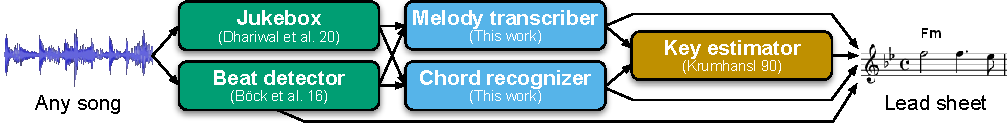
\includegraphics[width=\linewidth]{figs/sheetsage.pdf}
    \caption{
    % TODO: Clean this up. YouTube as input
    Inference procedure for Sheet Sage, our proposed system which transcribes any Western music audio into lead sheets (scores which depict melody as notes and harmony as chord names). The green, blue, and yellow boxes respectively take audio, features, and symbolic music data as input. Green boxes are modules that we built as part of this work---both are Transformers~\cite{vaswani2017attention} trained on their respective tasks using audio features from Jukebox~\cite{dhariwal2020jukebox} and data from \hooktheory~\cite{hooktheory}.
    %\pl{would it be possible to show a snippet of a lead sheet that we produce? might be pretty compelling}
    % CHRIS: There will be plenty in the sound examples!
    }
    \label{fig:sheet_sage}
    \vspace{-3mm}
\end{figure*}

Overall, using representations from \jukebox{} as input features results in stronger melody transcription performance than using either representations from \mtthree{} or conventional handcrafted features. 
Representations from both \mtthree{} and \jukebox{} outperform conventional handcrafted features, 
implying that both pre-training strategies are helpful for melody transcription. 
Note that these two pre-training approaches are compared holistically---these models differ on several axes 
(number of parameters, 
%number of dimensions, 
pre-training data semantics, 
pre-training task), 
and thus it is impossible to disentangle the individual contributions of these different factors without retraining the models. 
%We also note that fine tuning these models would likely be more effective than using their representations as input features\cite{???}

Qualitatively speaking, there is a noticeable difference in performance across the three different input features which correlates with quantitative performance (see~\cref{sound_examples} for sound examples). 
Using representations from \jukebox{} tends to result in fewer wrong notes than the other features, and substantially reduces the number of egregiously wrong notes (e.g.,~notes outside of the key signature). 
Representations from \jukebox{} also appear to aid in the detection of more nuanced rhythmic patterns. 
Moreover, using handcrafted features will often result in several repeated onsets during a longer sustained melody note---in contrast, using representations from \jukebox{} appears to mitigate this failure mode.

Different features also appear to complement one another to a degree. 
The strongest performance overall is obtained by combining all three features, though the improvement over \jukebox{} alone is marginal. 
%Combining \mtthree{} and \jukebox{} does improve performance over \jukebox{} alone, though only by a marginal amount. 
The practical downsides of combining all features outweigh the marginal benefits---running both pre-trained models effectively doubles the overall runtime, and the models have incompatible software dependencies. 
Hence, in the remainder of this paper we focus on models trained on individual features.
%Combining handcrafted features w/ either pre-trained approach has little effect on performance. 
% \pl{now that you mention computation, what are the different computation requirements, which matter for a practical system?}
% CHRIS: Good question, punting for later

\vspace{-1mm}
\subsection{Comparison to melody transcription baselines}
\label{sec:exp2}

We compare overall performance of our proposed melody transcription approach to several baselines. 
We evaluate all methods on a small subset of $10$ songs from RWC-MDB~\cite{goto2002rwc,goto2003rwc,goto2004development}, 
another dataset which includes melody transcription labels. 
We chose this specific subset in an effort to compare to early DSP-based work on melody transcription---none of the early approaches~\cite{paiva2004auditory,paiva2005detection,ryynanen2008automatic,weil2009automatic} shared code, however~\cite{ryynanen2008automatic} shared melody transcriptions for this $10$-song subset.

In addition to~\cite{ryynanen2008automatic}, we also compare to a baseline which applies a note segmentation heuristic~\cite{salamon2015midi} to a melody extraction algorithm~\cite{salamon2014melody}. 
We additionally compare to \mtthree{} in a zero-shot fashion---this model was not trained on melody transcription but was trained on some tasks which incorporate vocal transcription. 
Finally, because the vocals often carry the melody in popular music, we compare to a baseline of running the Tony~\cite{mauch2015computer} monophonic transcription software on source-separated vocals isolated with Spleeter~\cite{hennequin2020spleeter}. 
Because this approach will only work for vocals, we also separately report performance on a subset of our evaluation set where the vocals represent the melody. 
% It is worth noting that vocal isolation and transcription may be another promising path towards melody transcription, 
% as it is unclear the extent to which transcribing non-vocal melodies is essential for downstream applications.
Scores for all methods and baselines appear in~\Cref{tab:rwc_ryy}. 

Overall, our approach to training Transformers with features from \jukebox{} significantly outperforms the strongest baseline in both the vocals-only and unrestricted settings (${p < 0.01}$ using a two-sided t-test for paired samples). 
Qualitatively speaking, the stronger baselines produce transcriptions where a reasonable proportion of the notes are the correct pitches, but they have poor rhythmic consistency with respect to the ground truth. 
In contrast, our best model produces the correct pitches more often and with a higher degree of rhythmic consistency.
% Performance of our approach using different input representations is consistent with evaluation results on the \hooktheory{} test set. 